\chapter{Introduction}
\label{introduction}
\thispagestyle{plain}

In this world, most of the people think that Artificial Intelligence was created to simulate human behavior and the way we humans think. Even thought people are not wrong, Artificial Intelligence was also created to solve problems that humans are unable to solve, or to solve it in a shorter amount of time, with a better solution. For example, any exhaustive search requires pretty complex algorithms (heuristics, meta-heuristics etc) with complex mathematical functions in order to find a feasible solution. Problems humans may take days to find a feasible solution, or may not find a solution at all that fits its needs, algorithms like these may deliver a very good solution in minutes, hours or days, depending on how much time the human is willing to use in order to get a better solution and not just a feasible one. \\
\\
%%%%%%%%%%%%%%%
A concrete example is the creation of timetables for scheduling. Timetables can be used for educational purposes, sports scheduling, transportation timetabling etc. It may look like it's simple to create a timetable, but the truth is, this process normally requires following some rules in order to fit its purpose. These rules are called constraints in the timetabling subject, in which the more it has the harder it gets to create a feasible solution for the problem. In some cases, there are so many constraints in which some can be contradictory to each other, that it is needed to "relax the constraints" in order to solve the problem. \\
\\
%%%%%%%%%%%%%%%
The process of creating a timetable requires that the final solution follows a set of constraints. These can be divided in two groups: hard constraints and soft constraints. Hard constraints are a set of rules which must be followed in order to get a feasible solution. In the other hand, soft constraints may be called "optional" since there is no need to follow these to get a solution, because they are not mandatory. The quality of a solution is calculated by using these soft constraints. In another words: the more soft constraints a solution follows, the better it is. This quality is based on the points (weight) of the soft constraints that that solution didn't follow, so the more points, the worse the solution. The weight of each soft constraint is set by the one that created the constraints. \\
\\
%%%%%%%%%%%%%%%
Now that I talked a little bit about timetabling, let me specify the aim of this project. Its main is to create an examination timetable generator using ITC-2007 specifications. The solutions will be validated using a validator also created by me which specifies the quality of the solution and may do some corrections on the timetable in order to get an even better solution. It is also required that the final product may work with two test seasons which can be considered an extension to ITC-2007 formulation. In the end an (optional) Graphical User Interface will be created in order to allow the user to edit the current solution to fit the users needs and allow optimization to the edited solution. The generator will be tested using data from ITC-2007 and some actual data from six different programs presented in my university ISEL.\\
%%%%%%%%%%%%%%%
\section{Examination timetable: State of the Art}
\label{sec:sota}
In this topic we'll be writing about the state of art concerning examination timetable. Concretely, we'll be writing about why timetabling is a rather complex problem, some possible approaches on trying to solve a problem this type and some of the solutions already taken, specifically in ITC 2007.
%%%%%%%%%%%%%%%%%%%%
\subsection{Timetabling Problem}
%%%%%%%%%%%%%%%%%%%%
Timetabling is a subject that has been under investigation for more than ten years. There is no optimal solution for creating perfect timetables. Creating timetables is a process that requires complex algorithms in which search for solutions following a set of constraints, as mentioned above. These constraints can be divided into five main classes named Unary, Binary, Capacity, Event Spread and Agent constraints (REF: 2008 Rhydian Lewis)\\
\\
%%%%%%%%%%%%%%%
Timetabling problem may be formulated as a search or optimization problem (REF: 1999 Schaerf). Search problems consists about finding a solution that satisfies all the hard constraints, which soft constraints aren't the main goal, on contrary optimization problems are problems which tries to satisfy as most soft constraints as possible after satisfying all hard constraints. Optimization problems though are more commonly used to optimize feasible solutions obtained by using a search algorithm. The main goal consists in searching for a feasible solution which satisfies all hard constraints using a search algorithm. If the user's goal is to find the best solution possible in given time, a optimization solution may be applied to the solution given by the search algorithm.\\
\\
%%%%%%%%%%%%%%%
Search problems are quoted as NP-Complete (REF: NP-Complete wiki) and optimization problems are quoted as NP-Hard (REF: NP-Hard wiki) problem. Optimization problems are labeled NP-Hard because any optimization problem can be reduced to a graph coloring problem which is also NP-Hard. Graph coloring will be briefly explained later.\\
\\

\subsection{Solution approaches}
\label{subsection:SolutionsAppr}



\iffalse
Another tourist guide application with some interesting features is the GuidePal Offline City Guides~\cite{GuidePalWeb}\cite{GuidePaliPhone}. It allows users to download varied content for different cities and to consult information regarding restaurants, coffee shops, places to visit, and other attractions. Two screenshots of this application are illustrated on Figure~\ref{fig:guidePalIphoneScreenshots}.\\
\\
\begin{figure}
        \centering
        \begin{subfigure}[b]{0.25\textwidth}
                \centering
                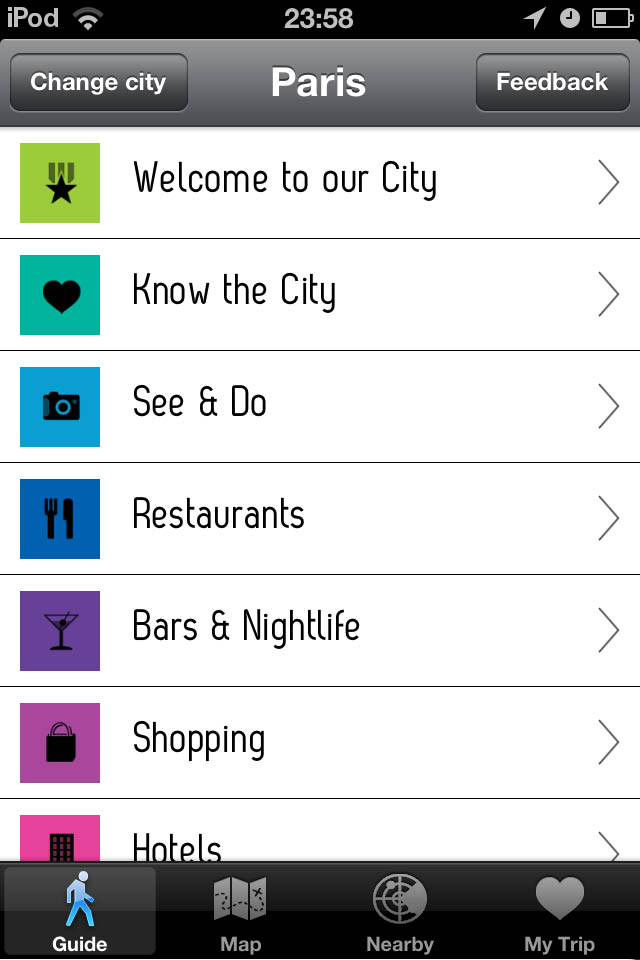
\includegraphics[height=7.5cm]{./images/screenshots/screenshot_guidepal_1.jpg}
                \caption{Category selection for filtering the locations.}
                \label{fig:guidePalCategorySelection}
        \end{subfigure}%
        \quad\quad\quad\quad\quad
        \begin{subfigure}[b]{0.25\textwidth}
                \centering
                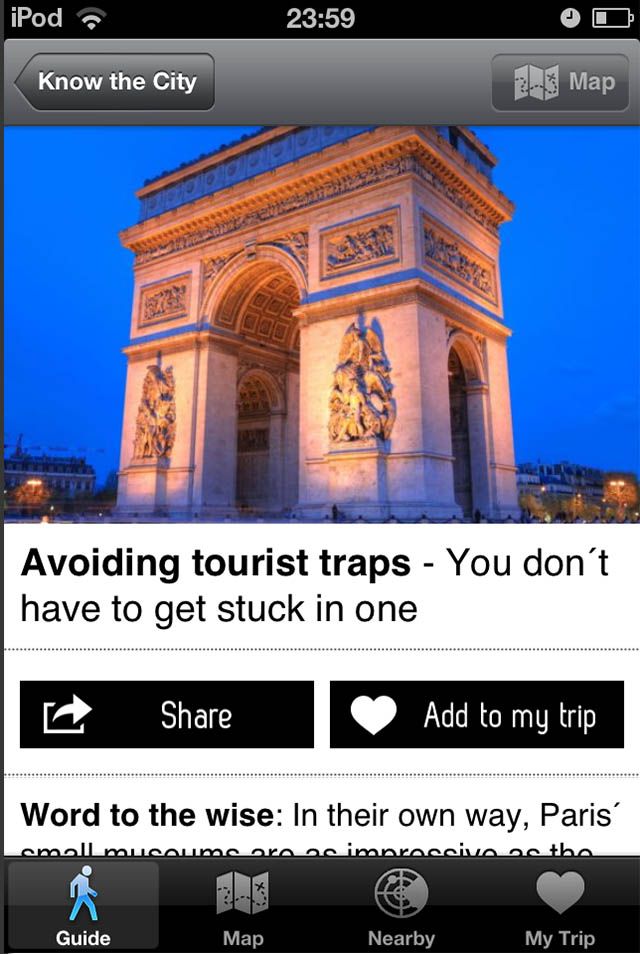
\includegraphics[height=7.5cm]{./images/screenshots/screenshot_guidepal_2.jpg}
                \caption{Detailed information about touristic location.}
                \label{fig:guidePalDetailedInformation}
        \end{subfigure}
        \caption{GuidePal~\cite{GuidePalWeb}\cite{GuidePaliPhone} iPhone application screenshots.}
        \label{fig:guidePalIphoneScreenshots}
\end{figure}
\\
In order to list the existing points of interest, the user selects the desired city and category as illustrated by  Figure~\ref{fig:guidePalIphoneScreenshots}~(\subref{fig:guidePalCategorySelection}). After selecting the intended category, a description for the point of interest is presented; Figure~\ref{fig:guidePalIphoneScreenshots}~(\subref{fig:guidePalDetailedInformation}) shows the selection of the "Know the City" category.\\
\\
This application also have some augmented reality features, providing users with the possibility to map the real world (captured by the camera of the device) with the touristic attractions in real time. When the camera points to the direction where touristic locations are available near by, those are presented above the image. By selecting any of the presented locations, the user is redirected to the detail page similar to one illustrated on Figure~\ref{fig:guidePalIphoneScreenshots}~(\subref{fig:guidePalDetailedInformation}).
%%%%%%%%
\subsection{mTrip}
mTrip~\cite{mTrip} travel guide service is mainly used for big cities such as Paris, Berlin,  Madrid, and others. It is available as a separate application for each one of the major cities (for both iPhone and Android) and allows people to consult information regarding points of interest without an Internet connection. Figure~\ref{fig:mtripScreenshots} presents some screenshots of this application. \\
\\
Users can plan an itinerary or create guides for the cities by providing the detailed information on the touristic attractions they plan to visit. After specifying the dates for the trip, each user can manually compose his itinerary or allow mTrip to automatically generate an itinerary for the trip. When the automatic mode is chosen, one must indicate preferences for the attractions to be visited, as shown on Figure~\ref{fig:mtripScreenshots}~(\subref{fig:mTripPreferencesCustomization}). A list of points of interest is presented when the user selects a specific category, similar to those shown on Figure~\ref{fig:mtripScreenshots}~(\subref{fig:mTripTouisticLocations}).
\\
%%%%%%%%%%%%%%%%%
\begin{figure}
        \centering
        \begin{subfigure}[b]{0.25\textwidth}
                \centering
                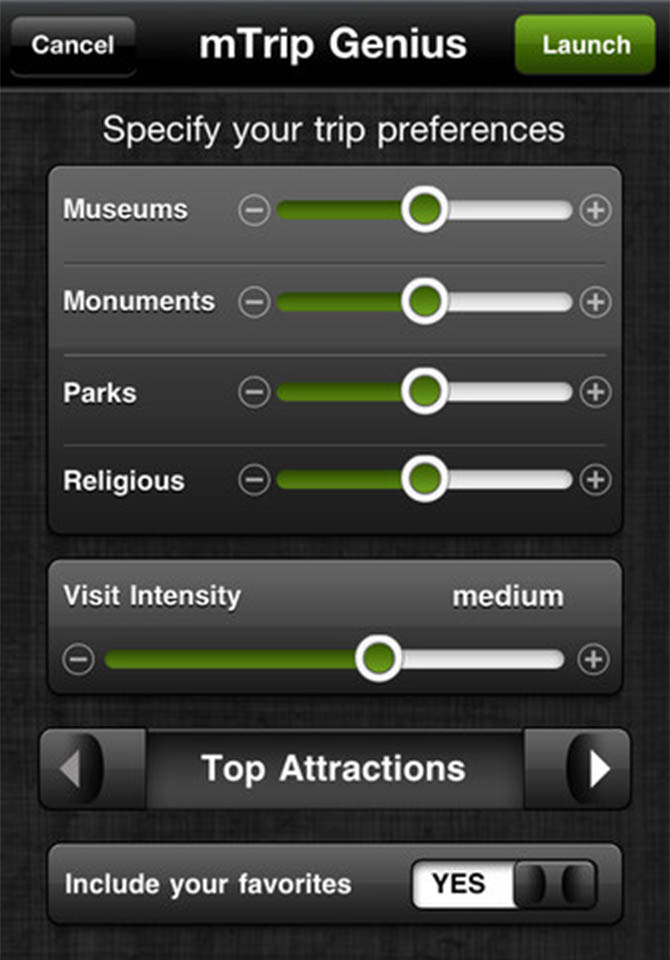
\includegraphics[height=7.5cm]{./images/screenshots/screenshot_mtrip_1.jpg}
                \caption{Customization of the itinerary.}
                \label{fig:mTripPreferencesCustomization}
        \end{subfigure}%
        \quad\quad\quad\quad\quad\quad
        \begin{subfigure}[b]{0.25\textwidth}
                \centering
                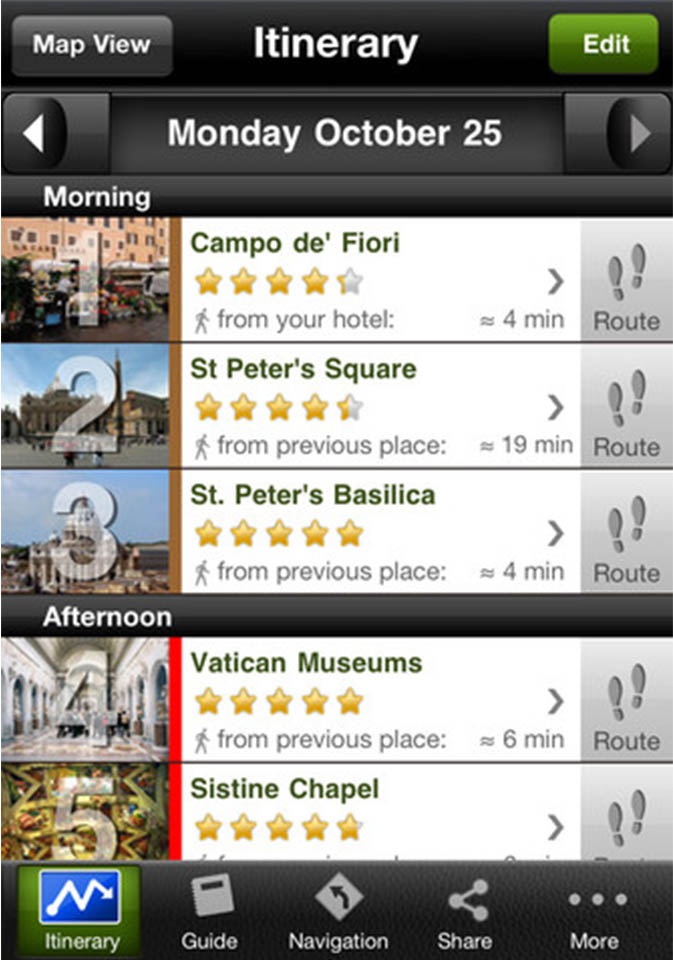
\includegraphics[height=7.5cm]{./images/screenshots/screenshot_mtrip_2.jpg}
                \caption{List of the touristic locations.}
                \label{fig:mTripTouisticLocations}
        \end{subfigure}
        \caption{mTrip iPhone application screenshots.}
        \label{fig:mtripScreenshots}
\end{figure}
\\
%%%%%%%%%%%%%%%%%
Each point of interest is accompanied by a description, a photo, opening hour, prices, as well as the comments and ratings from other travellers. The application provides an augmented reality tool that allows to preview of the points of interest around the user's current location.
%%%%%%%%
\subsection{Triposo}
Triposo~\cite{triposo} shares similar concepts with the mTrip application. However, it includes much more countries as well as smaller cities. When one picks the country to visit, the download of information regarding the points of interest for that country starts immediately, allowing to consult this information later in offline mode. Some major cities require additional downloads due to the large amount of the points of interest and touristic attractions. For big cities, users have access to special information regarding the city guide about all sights, a list of restaurants and extended nightlife options. The application also offers a travel dashboard with currency converter, weather, and useful native language phrases. Triposo uses freely available content from different sources, such as Wikipedia~\cite{wikipedia}, Wikitravel~\cite{wikitravel}, World66~\cite{world66}, among others.\\
\\
As it is shown by the screenshot on Figure~\ref{fig:triposoScreenshots}~(\subref{fig:triposoSuggestedPointsOfInterest}), a set of suggested points of interest for Lisbon is presented along with the main navigation items. Figure~\ref{fig:triposoScreenshots}~(\subref{fig:triposoWeahtherTime}) shows the current weather and current time for Porto as well as the spelling of some Portuguese words.\\
%%%%%%%%%%
\begin{figure}
        \centering
        \begin{subfigure}[b]{0.25\textwidth}
                \centering
                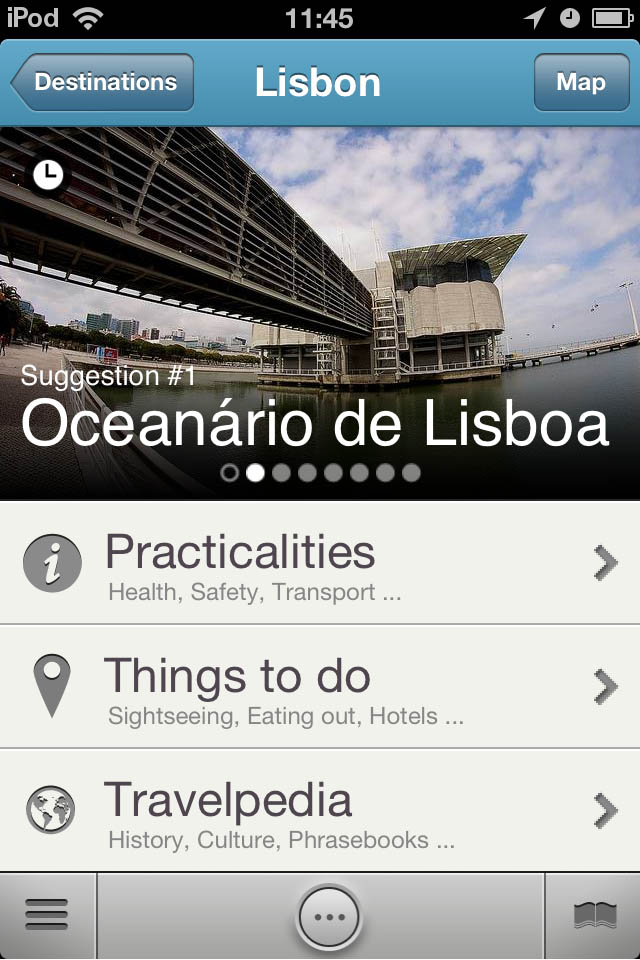
\includegraphics[height=7.5cm]{./images/screenshots/screenshot_triposo_1.jpg}
                \caption{Suggested points of interest.}
                \label{fig:triposoSuggestedPointsOfInterest}
        \end{subfigure}%
        \quad\quad\quad\quad\quad
        \begin{subfigure}[b]{0.25\textwidth}
                \centering
                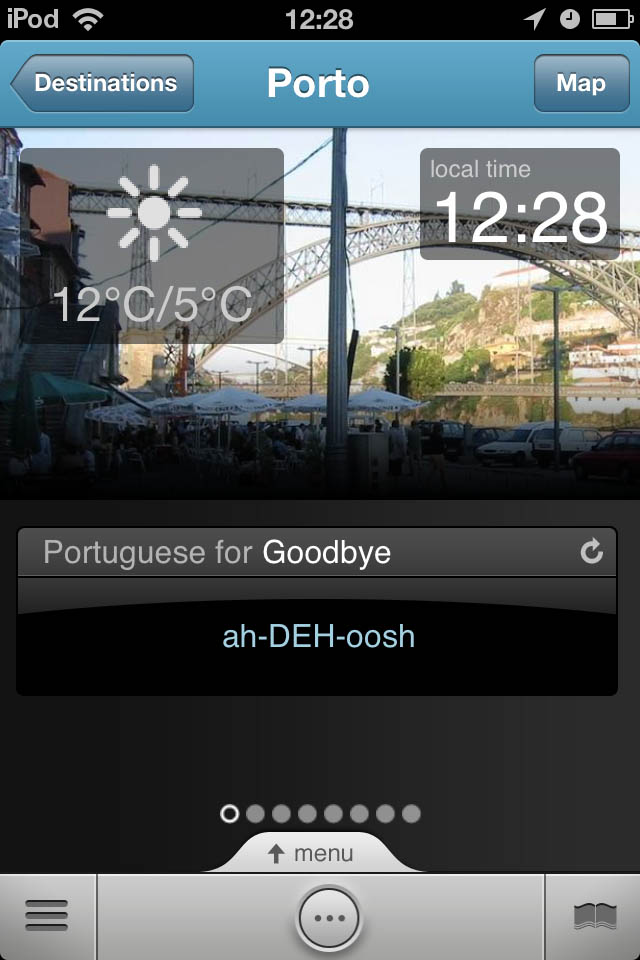
\includegraphics[height=7.5cm]{./images/screenshots/screenshot_triposo_2.jpg}
                \caption{Shortcuts and useful information.}
                \label{fig:triposoWeahtherTime}
        \end{subfigure}%
        \caption{Triposo iPhone application screenshots.}
        \label{fig:triposoScreenshots}
\end{figure}


%%%%%%%%%%
\subsection{Foursquare}
Foursquare is a service that allows registered users to "check-in\footnote{Check-in refers to the user's action for posting his current location at a venue.}" at their current location. It is composed by both web and mobile applications for iPhone, Android and Blackberry. Users with special permission have the possibility to contribute with new locations, such as coffee shops, restaurants, sights, among others. The service was created in 2009 and in March of 2011 a new version with a recommendation engine~\cite{foursqureRecommendationEngine} was developed, for suggesting places that users might like, based on their past actions.\\
\\
In 2013 an updated version of the service was launched, where users can consult the sights nearby their current location. The map view with the recommended sights nearby users current location is shown on Figure~\ref{fig:4SqureScreenshots}~(\subref{fig:4squre2}). An example of the touristic location details is shown on Figure~\ref{fig:4SqureScreenshots}~(\subref{fig:4squre3}) where user can have the preview of the location, save it to favourites, perform the check in, among others.\\
\\
\begin{figure}
        \centering
        \begin{subfigure}[b]{0.25\textwidth}
                \centering
                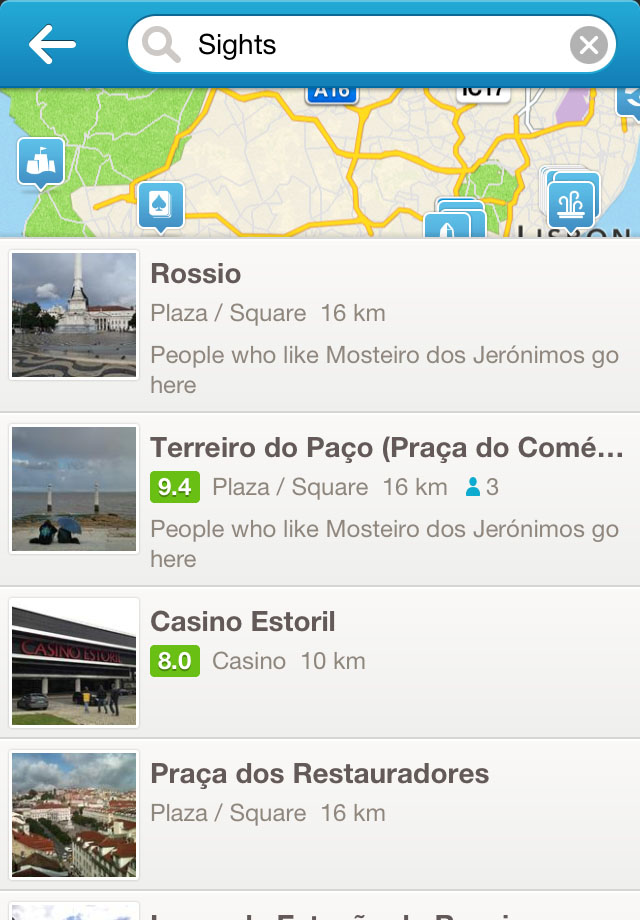
\includegraphics[height=7cm]{./images/screenshots/screenshot_foursqure_1.jpg}
                \caption{Map view with sights nearby user's location.}
                \label{fig:4squre2}
        \end{subfigure}%
        \quad\quad\quad\quad\quad
        \begin{subfigure}[b]{0.25\textwidth}
                \centering
                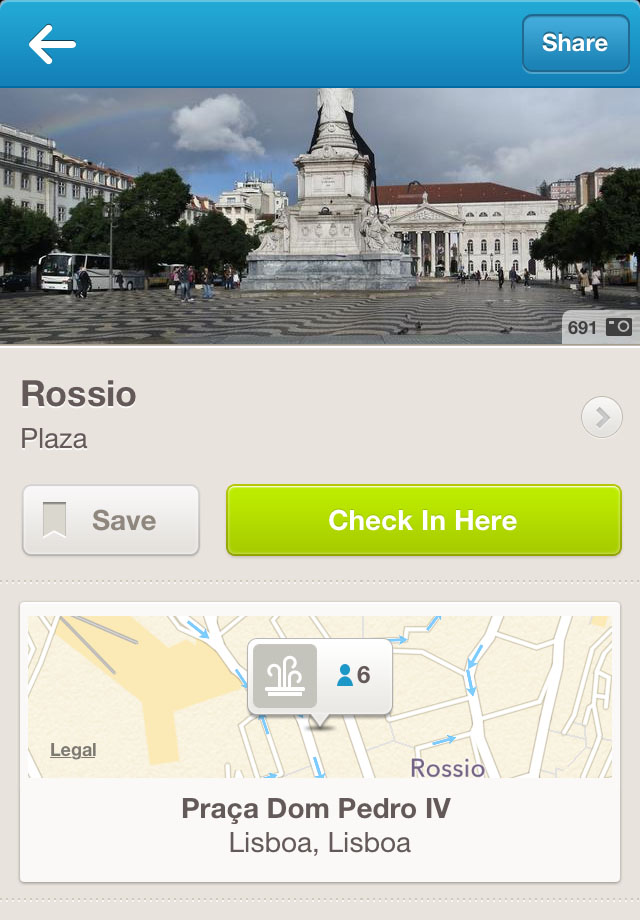
\includegraphics[height=7cm]{./images/screenshots/screenshot_foursqure_2.jpg}
                \caption{Details of the Touristic location.}
                \label{fig:4squre3}
        \end{subfigure}%
        \caption{Foursquare iPhone application screenshots.}
        \label{fig:4SqureScreenshots}
\end{figure}
\\
All these applications are modern solutions for tourist guides. The Foursquare service was created in 2009, the mTrip and TouristEye in 2010, whereas the Triposo and GuidePal have been published in 2011. 
\newpage

\section{Proposed Solution}
\label{sec:ftbd}
This Section introduces the simplified service architecture as well as the employed technologies used during the development of the system components. The system is mainly composed by the~\gls{rest}~\cite{RestWebber} service with a data access layer which exposes a set of endpoints\footnote{In \gls{soa}, an endpoint is the entry point to a service.} accessible by the client applications. Client applications are available as Web-based and Mobile (for iOS~\cite{ios} platforms iPhone and iPad). Figure~\ref{fig:introductioArchitecture} shows the proposed service architecture.\\
\\
\begin{figure}[h!]
 \centering
   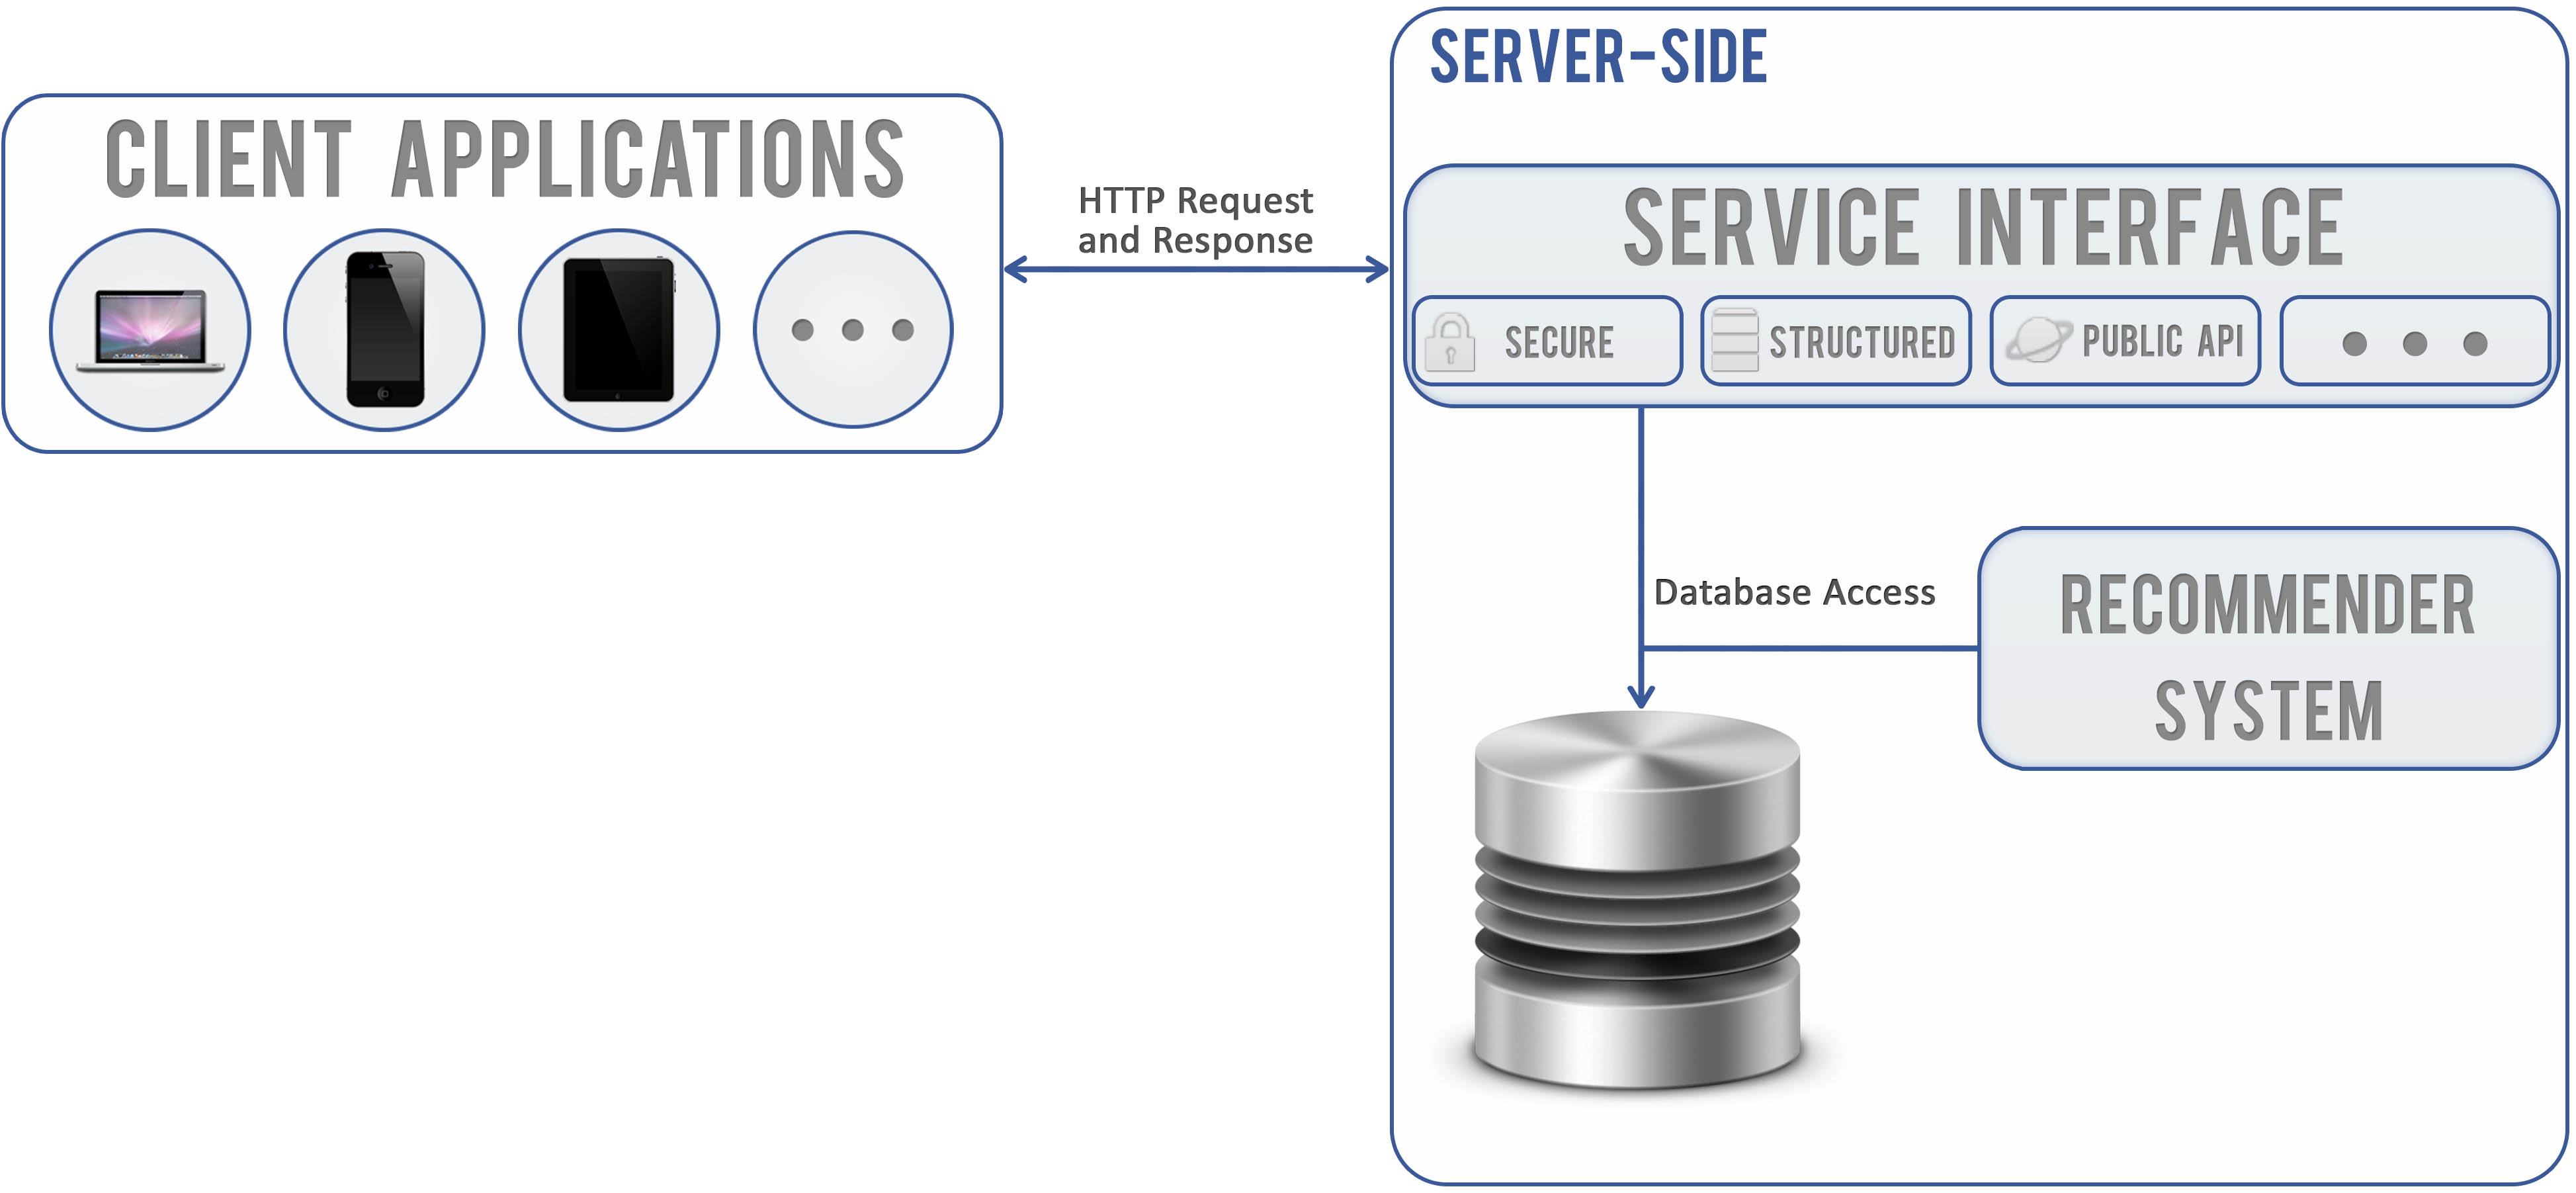
\includegraphics[width=14.8 cm]{./images/diagrams/diagram_introduction_architecture.jpg}
   \caption{Generic service architecture.}
   \label{fig:introductioArchitecture}
\end{figure}\\
\\
The service is divided into four main layers, with the following roles:
\begin{itemize}
 \item The Database layer stores information regarding points of interest, user data, among other types of data.
 \item The Service Interface is responsible for communicating with the Database layer. It makes all accesses transparent to the end client applications. This layer is mainly responsible for the data security and integrity, delivery of information in structured format, among others.
 \item The Recommender System is responsible for finding new points of interest based on the user's past actions, and to recommend these to the user. This service uses data from the database layer in order to compute recommendations.
 \item Client Applications make \gls{http} requests in order to access data from the public \gls{api}, provided by the Service Interface layer.
\end{itemize}

\subsection{Tools and Technologies}
\label{subsec:ttbuipd}
This Subsection introduces the technologies and tools used to achieve the goals of this project. We begin by describing a set of technologies related to databases, data model, and the \gls{rest} service. Then, the Web related technologies are discussed and finally we address the mobile applications.\\
\\
%%%%
For information storage, we use the MySQL~\cite{MySqlOrcale} relational database, which uses the \gls{sql} for accessing and manipulating databases. In order to facilitate the service development process, a pre-populated database was created with a few tens of points of interest.\\
\\
%%%%
The \gls{rest}~\gls{api} is developed in order to provide a single data source for client applications, including those already developed within this project and others that may appear in the future. The \gls{api} is implemented using the Java environment and Play~Framework~\cite{playFramework}.\\
\\
The Web application implementation is focused in technologies for user interface definition and structuring such as~\gls{html5}~\cite{html5},~\gls{css3}~\cite{css3} and also the JavaScript~\cite{javaScript} technology to enrich user's interactivity. The server side of the web application was developed using the Play Framework. Twitter Bootstrap~\cite{twitterBootstrap} framework was used to generate the layout with desired dynamic content, thus providing an user friendly platform.\\
\\
%\marginpar{} %%%
In the past few years, mobile devices have been used and widespread with great success, starting with Apple's iPhone launch and later with the iPad~\cite{iPadSanchez}. Both devices share the same operating system named iOS that offers a development platform for object-oriented applications. Those are written in Objective-C~\cite{ObjectiveC}\footnote{The Objective-C is a computer programming language based on C and Smalltalk. It is designed to leverage the C language with full object-oriented programming capability, through the mechanism of message passing. When in Objective-C one sends a message, its target is resolved at runtime and then it interprets the message with the receiving object~\cite{ObjectiveC}~\cite{objectiveCBook}.} using the iOS SDK (Software Development Kit). In the course of this project the targeted applications were designed taking into consideration advanced aspects of the iOS platform such as sharing code between iPhone and iPad, by means of an Universal Application~\cite{UniversalApps}.\\
\\
%\marginpar{} %%%
The development of these applications was carried out using the \gls{ide} Xcode~\cite{Xcode}.

\subsection{Core Features}
\label{subsec:cf}
This Subsection contains a description of the core features provided by the service, which are presented in Table~\ref{tab:coreFeatures}.\\
\\
\newpage
\begin{center}
    \begin{longtable}{ | p{3.5cm} | p{11.1cm} |}
    \caption{Core features of the GuideMe service.}
    \label{tab:coreFeatures}
	\\
    \hline
    \textbf{Feature Name} & \textbf{Description}\\ \hline
    \hline
    \specialcell[t]{Internationalization\\support} & 
    The aim of the project is to support points of interest of Portugal, but its architecture is designed in order to easily be expanded and to support other countries. Multilingual support is implemented for the database, REST API and application levels. \\ 
    \hline
    
    Filtering options &
    The following features are supported:
	\begin{itemize}
	\item lookup for points of interest nearby the user's current location;
	\item filtering of the locations based on the following characteristics:
	\begin{itemize}
		\item specific attraction;
		\item user's current location, by using the geographic coordinates retrieved from the mobile device;
		\item time that the user can spend;
		\item time of day of the visit;
		\item preferred weather conditions.
	\end{itemize}
	\item places that can be visited under given weather conditions such as rainy or sunny days, among others. It requires integration with the \gls{wwo} meteorology~\gls{api}, in order to advise or not the visit to the chosen user location;
	\item filtering by the maximum distance to the point of interest, based on the user's current location and mobility.
	\end{itemize}
    \\ 
    \hline
    
    \specialcell[t]{Wanted and\\already seen} &
	Users have the possibility to create a list of locations that they intend to visit as well as access the history of already visited locations. \\ 
    \hline

	\specialcell[t]{Social component} &
    	The following features are supported:
	\begin{itemize}
	\item Integration with social networks in order to encourage users to share visits with their friends;
	\item Based on the visits and mutual preferences between various users, the system recommends new places to visit that users may like. The recommendations are produced by the recommender system, using Collaborative Filtering (CF)~\cite{ibCollabrativeVSGK}\cite{AmazonRecommendGLBSJY}\cite{recommSystemPMVS} algorithms. The proposed solution is further explained in Section~\ref{sec:ocft};
	\item The service implements the social component by itself, providing the concept of the \emph{Following} and \emph{Follower} in order to establish friendship between users. Users are notified about certain actions performed by their friends.
	\end{itemize}
    \\ 
    \hline
    
    Notification system &
    Users can receive push notifications on their iOS device when someone has started to follow them. These notifications are carried out using the~\gls{apns}~\cite{apns}.\\
\hline
    
   	Login and sign up &
    Authentication and sign up through the most popular social network services, such as Facebook~\cite{FacebookLogin} and Twitter~\cite{TwitterLogin}. \\
    \hline
    
   	Back office &
    The iOS applications implements a back office system where privileged users can create or edit an existing location. They have permission to consult log information of the different service components, to analyse and correct information regarding the touristic location that were reported by other users.\\
\hline

   	Near by  &
    Preview of the sights, near by user's geographic locations. The use-case of this feature is illustrated on Figure~\ref{fig:useCaseFilterByLocation}.\\
\hline

   	Recommended touristic locations  &
	The service performs recommendation of the touristic locations to users, based on their past visits. The detailed illustration of this scenario is shown on Figure~\ref{fig:useCaseRecommendationLocation}.\\
\hline
    \end{longtable}
\end{center}
%%%%%%%%%%%%%%%%%%%%
The use-case illustrated on Figure~\ref{fig:useCaseFilterByLocation} consists in providing the user with information regarding the sights near by his/her current location.\\
%%%%%%%%%%%%%%%%%%%%
\begin{figure}[h!]
 \centering
   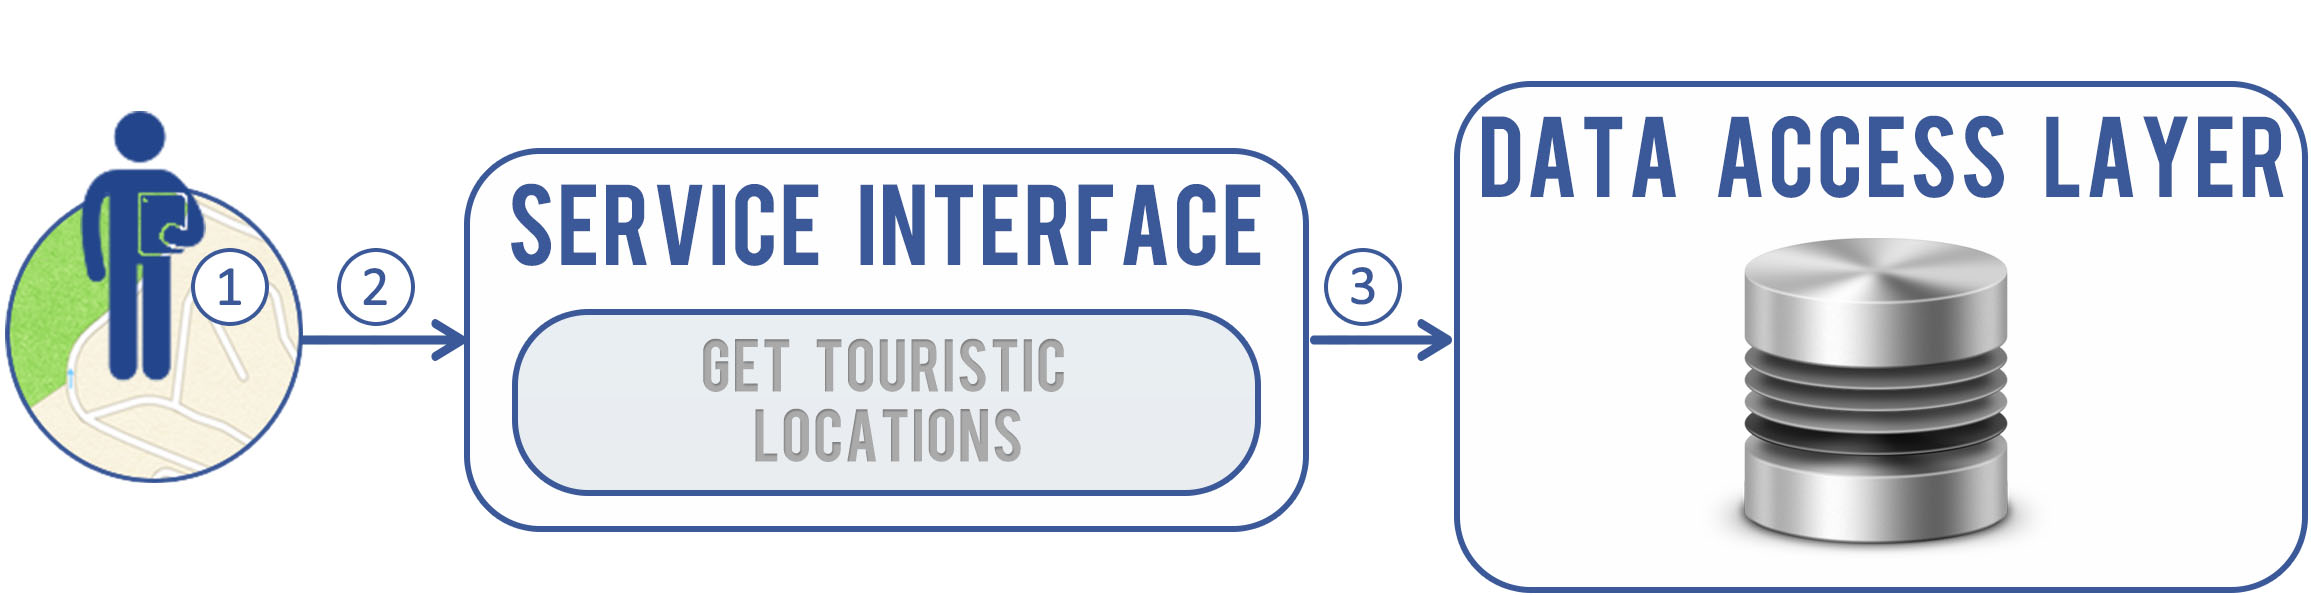
\includegraphics[width=13.0 cm]{./images/diagrams/diagram_usecase_users_location.jpg}
   \caption{Use-case of the near by feature.}
   \label{fig:useCaseFilterByLocation}
\end{figure}\\
%%%%%%%%%%%%%%%%%%%%
Each step is detailed as follows:
\begin{enumerate}
\item The geographic coordinates of user's current location, are obtained through the ~\gls{gps} of the mobile device.
\item Through the service interface, users make the requests to obtain the touristic locations passing the previously obtained geographic coordinates.
\item The service interface interacts with the Data Access Layer (DAL) in order to list the touristic locations. The distance is calculated between each sight and the submitted geographic coordinates, providing the results sorted in ascending order of distance.
\end{enumerate}
%%%%%%%%%%%%%%%%%%%%
The recommender system is one of the most important features of the developed service. The summarised process of the recommendation system is illustrated on Figure~\ref{fig:useCaseRecommendationLocation}.\\
%%%%%%%%%%%%%%%%%%%%
\begin{figure}[h!]
 \centering
   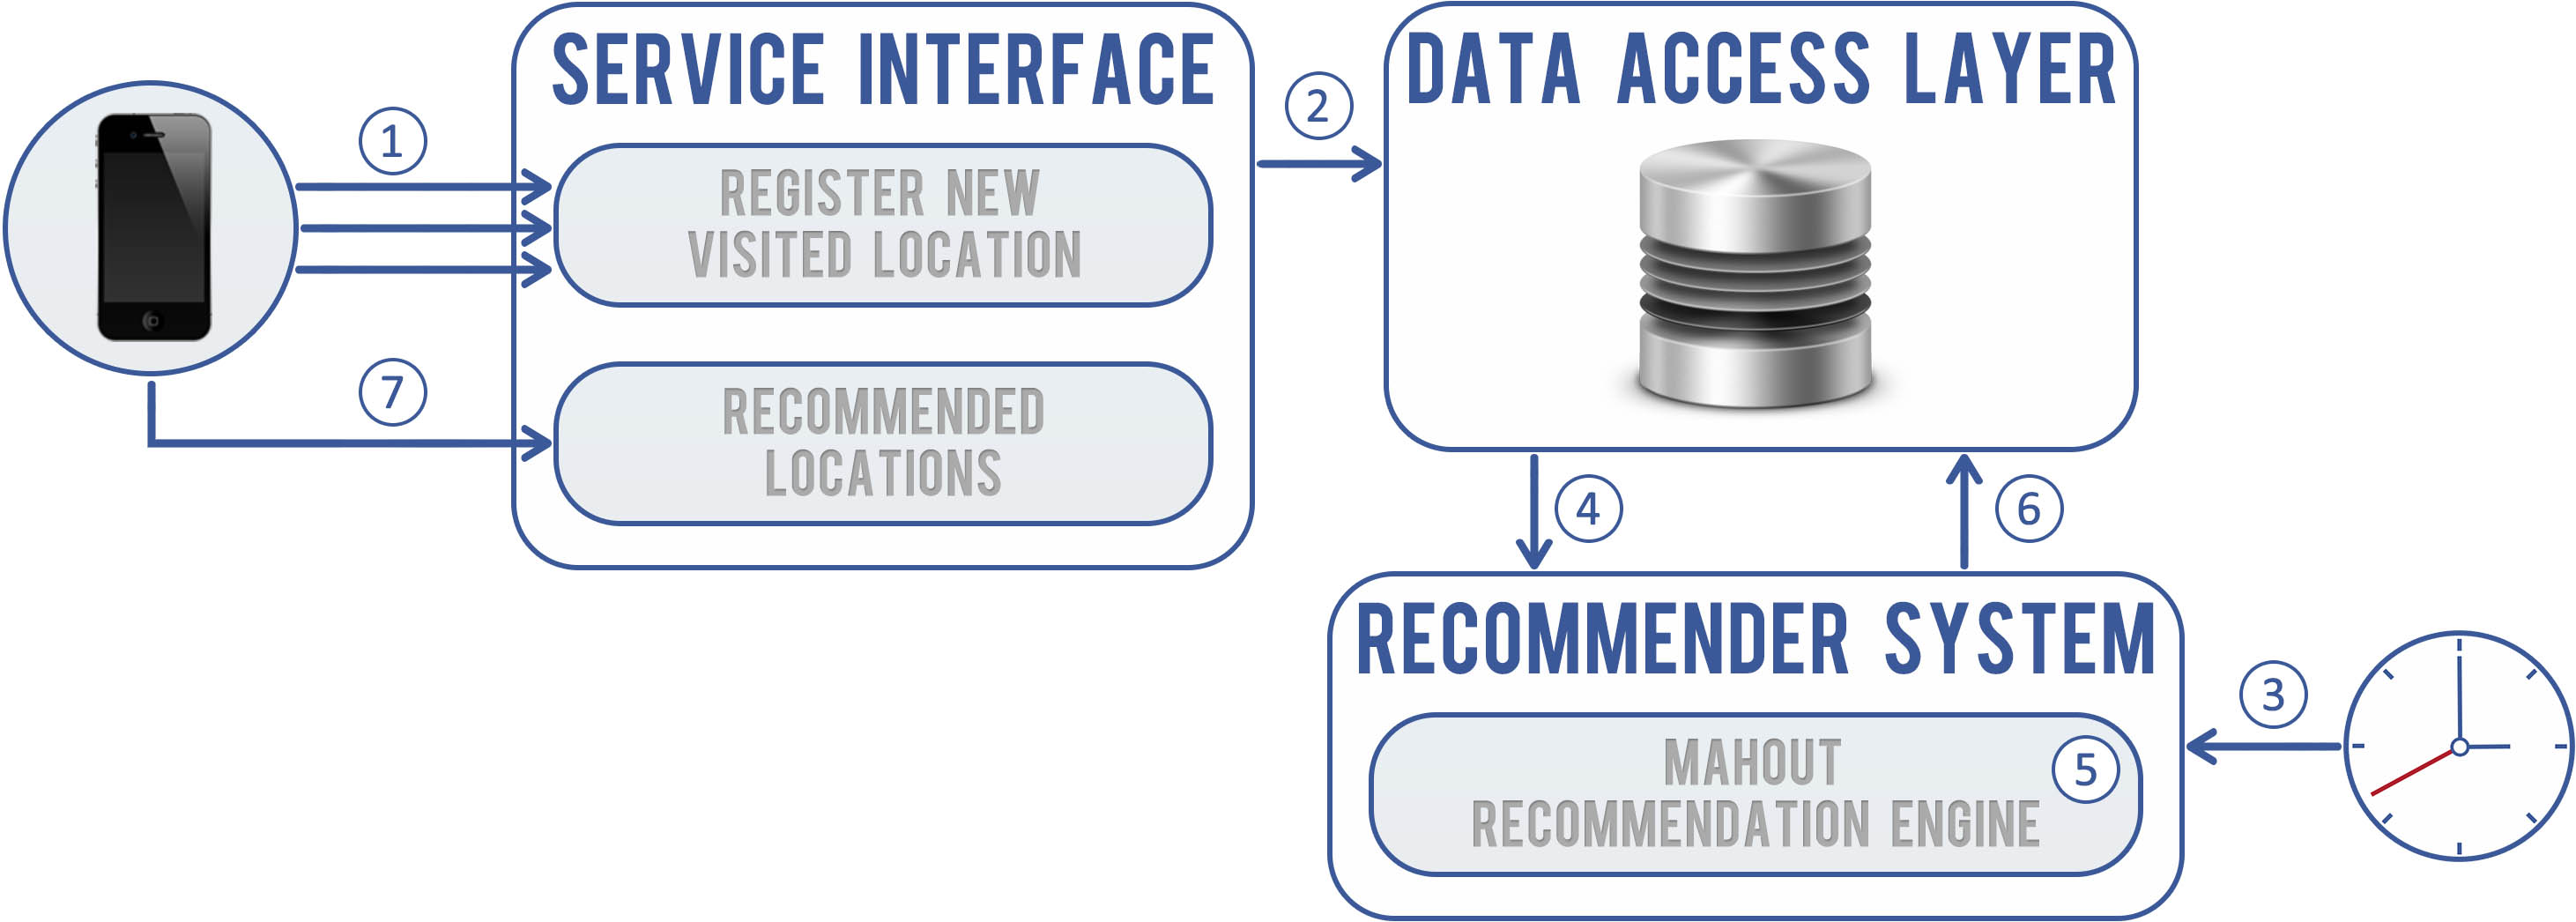
\includegraphics[width=13.0 cm]{./images/diagrams/diagram_usecase_recommender_system.jpg}
   \caption{The recommendation process.}
   \label{fig:useCaseRecommendationLocation}
\end{figure}\\
The full process of the recommendation system is as follows:
\begin{enumerate}
\item Through the service interface, the user marks new locations as visited.
\item Using the implemented DAL, the information is stored into the database.
\item The Cron Job\footnote{Cron is a time-based job scheduler in Unix-like computer operating systems.}~\cite{cronTab} is triggered everyday at 3:00 A.M., performing the recommendation process.
\item The recommender system obtains users eligible for the new recommendations.
\item For each user, the recommender system computes a set of locations previously unseen by the user.
\item Through the DAL, the recommender service removes previous recommendations and populates the database with the new information.
\item Later, the user obtains a list of recommendations through the service interface.
\end{enumerate}
%%%%%%%%%%%%%%%%%%%%
When comparing the GuideMe service with similar applications reviewed in Section~\ref{sec:sota}, it offers:
\begin{itemize}
	\item filters of unique kind that allow searching for points of interest;
	\item a friendly and usable interface for both Web and mobile applications;
	\item integration with algorithms and services that minimize human interaction during the approval process of newly inserted locations.
\end{itemize}

\section{Report Organization}
\label{sec:reportOrganization}
The remainder of this report is organized as follows. In Chapter~\ref{theory}, we introduce the background concepts and terminology of the recommender system and different collaborative filtering techniques. Chapter~\ref{implementation} approaches the proposed solution by detailing: the chosen service architecture, the integration with the~\gls{apns} service, the analysis of different frameworks for the implementation of the~\gls{dal}, and the~\gls{rest}~\gls{api}. Chapter~\ref{implementation} also includes prototypes that were initially designed before the development of the client applications.\\
\\
In Chapter~\ref{developed-work}, we describe all the developments that were made for making this project a reality. In detail, this Chapter describes the implementation aspects of the database models for both Service and Log databases, structure of the the~\gls{rest}~\gls{api} endpoints, different characteristics of the implemented recommender system, and push notification provider. We introduce the main features, as also some implementation details of the web and iOS applications. Chapter~\ref{chapter:expRsults} is devoted to the experimental results, which have guided the implementations in the correct direction. This Chapter reflects an analysis of the different recommendation system algorithms and load tests.\\
\\
We end the document with the Chapter~\ref{conclusions} by detailing the core aspects of the project and the fulfilled objectives. In order to make the service more usable and robust, as future work we present some points that should be improved in terms of security and functionalities.

\section{Our Contribution}
\label{sec:ourContribution}
We've recently submitted an article~\cite{guideMeArticle} to the 2013 Conference on Electronics, Telecommunications and Computers (CETC 2013), where we describe the main parts of this work. We believe that the developed project contribute to the evolution of tourist guide services, and promotes the effective integration of recommendation systems as a tool to easily find new interesting places to visit.
\fi